\documentclass[border=10pt]{standalone}
\usepackage{pgfplots}
\usepackage{pgfplotstable}
\usepackage{tikz}
\pgfplotsset{compat=1.18}
\usetikzlibrary{positioning, calc}

% 定义颜色（与原图匹配）
\definecolor{colorBlue}{RGB}{79, 150, 183}
\definecolor{colorPurple}{RGB}{177, 87, 127}
\definecolor{colorOrange}{RGB}{243, 162, 41}
\definecolor{colorRed}{RGB}{204, 85, 88}
\definecolor{colorGreen}{RGB}{130, 172, 98}
\definecolor{colorBrown}{RGB}{163, 118, 93}

\begin{document}

% ============================================================================
% 图 1: Comparison with Traditional BFT Consensus Algorithms
% ============================================================================
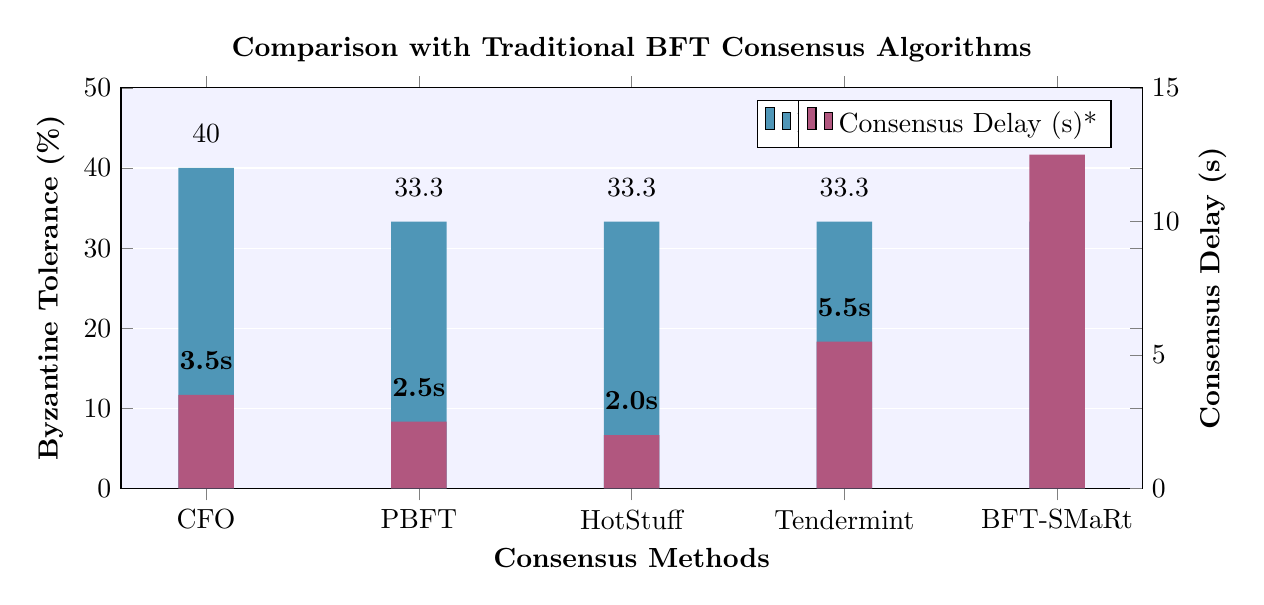
\begin{tikzpicture}
\begin{axis}[
    title={\textbf{Comparison with Traditional BFT Consensus Algorithms}},
    symbolic x coords={CFO, PBFT, HotStuff, Tendermint, BFT-SMaRt},
    xtick=data,
    xlabel={\textbf{Consensus Methods}},
    ylabel={\textbf{Byzantine Tolerance (\%)}},
    ybar,
    bar width=20pt,
    width=1.2\textwidth,
    height=0.55\textwidth,
    ymin=0, ymax=50,
    ymajorgrids=true,
    grid style={white},
    axis background/.style={fill=blue!5},
    legend pos=north east,
    every node near coord/.append style={font=\bfseries, yshift=2mm},
    nodes near coords,
]
% Byzantine Tolerance
\addplot[fill=colorBlue, draw=none] coordinates {
    (CFO, 40.0) (PBFT, 33.3) (HotStuff, 33.3) (Tendermint, 33.3) (BFT-SMaRt, 33.3)
};
\addlegendentry{Byzantine Tolerance (\%)}
\end{axis}

\begin{axis}[
    symbolic x coords={CFO, PBFT, HotStuff, Tendermint, BFT-SMaRt},
    xtick=data,
    ylabel={\textbf{Consensus Delay (s)}},
    ybar,
    bar width=20pt,
    width=1.2\textwidth,
    height=0.55\textwidth,
    ymin=0, ymax=15,
    axis y line*=right,
    y axis line style={opacity=0},
    ylabel style={anchor=north},
    axis x line=none,
    every node near coord/.append style={font=\bfseries, yshift=2mm, anchor=south},
    nodes near coords,
    point meta=explicit symbolic,
    legend pos=north east,
]
% Consensus Delay
\addplot[fill=colorPurple, draw=none, point meta=explicit symbolic] coordinates {
    (CFO, 3.5) [3.5s]
    (PBFT, 2.5) [2.5s]
    (HotStuff, 2.0) [2.0s]
    (Tendermint, 5.5) [5.5s]
    (BFT-SMaRt, 12.5) [12.5s]
};
\addlegendentry{Consensus Delay (s)*}
\end{axis}
\end{tikzpicture}

\vspace{1cm}

% ============================================================================
% 图 2(a): Prediction Accuracy Comparison (Horizontal Bar Chart)
% ============================================================================
\begin{tikzpicture}
\begin{axis}[
    title={\textbf{(a) Prediction Accuracy Comparison}},
    xbar,
    bar width=22pt,
    width=0.6\textwidth,
    height=0.55\textwidth,
    xmin=75, xmax=100,
    xmajorgrids=true,
    grid style={white},
    axis background/.style={fill=blue!5},
    symbolic y coords={Bulyan, Multi-Krum, Median, Trimmed Mean, Krum, CFO},
    ytick=data,
    yticklabel style={font=\small},
    xlabel={\textbf{Average Accuracy (\%)}},
    every node near coord/.append style={font=\bfseries, anchor=west, xshift=2mm},
    nodes near coords,
    nodes near coords align={horizontal},
]
\addplot[fill=colorBlue, draw=black, thick] coordinates {(94.1, CFO)};
\addplot[fill=colorOrange, draw=black, thick] coordinates {(85.0, Krum)};
\addplot[fill=colorRed, draw=black, thick] coordinates {(80.0, Trimmed Mean)};
\addplot[fill=colorGreen, draw=black, thick] coordinates {(80.0, Median)};
\addplot[fill=colorRed!70, draw=black, thick] coordinates {(90.0, Multi-Krum)};
\addplot[fill=colorBrown, draw=black, thick] coordinates {(88.0, Bulyan)};
\end{axis}
\end{tikzpicture}

\vspace{1cm}

% ============================================================================
% 图 2(b): Tolerance vs Accuracy (Scatter Plot)
% ============================================================================
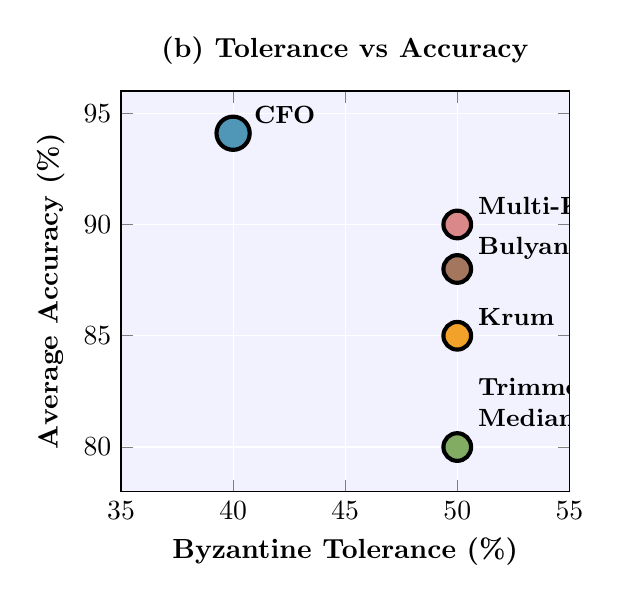
\begin{tikzpicture}
\begin{axis}[
    title={\textbf{(b) Tolerance vs Accuracy}},
    width=0.6\textwidth,
    height=0.55\textwidth,
    xmin=35, xmax=55,
    ymin=78, ymax=96,
    xmajorgrids=true,
    ymajorgrids=true,
    grid style={white},
    axis background/.style={fill=blue!5},
    xlabel={\textbf{Byzantine Tolerance (\%)}},
    ylabel={\textbf{Average Accuracy (\%)}},
]
% CFO
\filldraw[fill=colorBlue, draw=black, line width=1.5pt] (axis cs:40, 94.1) circle (6pt);
\node[anchor=south west, font=\bfseries\small] at (axis cs:40.5, 94.1) {CFO};
% Multi-Krum
\filldraw[fill=colorRed!70, draw=black, line width=1.5pt] (axis cs:50, 90.0) circle (5pt);
\node[anchor=south west, font=\bfseries\small] at (axis cs:50.5, 90.0) {Multi-Krum};
% Bulyan
\filldraw[fill=colorBrown, draw=black, line width=1.5pt] (axis cs:50, 88.0) circle (5pt);
\node[anchor=south west, font=\bfseries\small] at (axis cs:50.5, 88.0) {Bulyan};
% Krum
\filldraw[fill=colorOrange, draw=black, line width=1.5pt] (axis cs:50, 85.0) circle (5pt);
\node[anchor=south west, font=\bfseries\small] at (axis cs:50.5, 85.0) {Krum};
% Trimmed Median
\filldraw[fill=colorGreen, draw=black, line width=1.5pt] (axis cs:50, 80.0) circle (5pt);
\node[anchor=south west, font=\bfseries\small, align=left] at (axis cs:50.5, 80.5) {Trimmed\\Median};
\end{axis}
\end{tikzpicture}

\vspace{1cm}

% ============================================================================
% 图 3: Comparison with Multi-Agent Consensus Methods
% ============================================================================
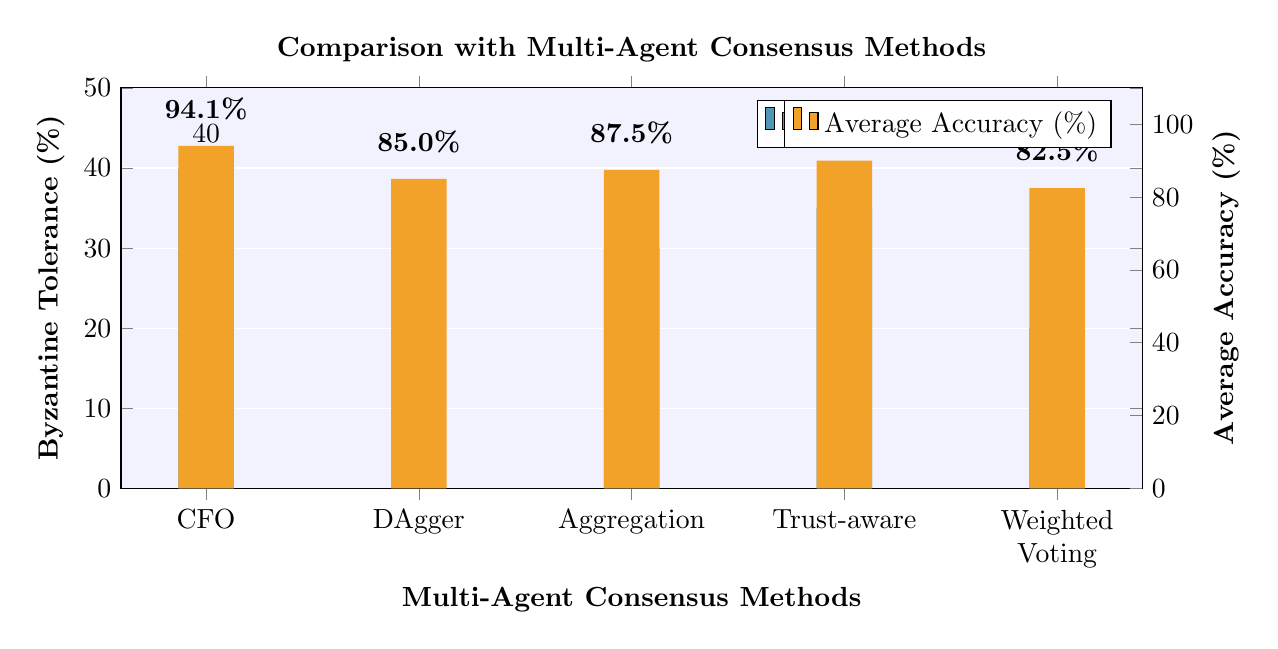
\begin{tikzpicture}
\begin{axis}[
    title={\textbf{Comparison with Multi-Agent Consensus Methods}},
    symbolic x coords={CFO, DAgger, Aggregation, Trust-aware, Weighted Voting},
    xtick=data,
    xlabel={\textbf{Multi-Agent Consensus Methods}},
    ylabel={\textbf{Byzantine Tolerance (\%)}},
    ybar,
    bar width=20pt,
    width=1.2\textwidth,
    height=0.55\textwidth,
    ymin=0, ymax=50,
    ymajorgrids=true,
    grid style={white},
    axis background/.style={fill=blue!5},
    legend pos=north east,
    every node near coord/.append style={font=\bfseries, yshift=2mm},
    nodes near coords,
    x tick label style={text width=2cm, align=center},
]
% Byzantine Tolerance
\addplot[fill=colorBlue, draw=none] coordinates {
    (CFO, 40) (DAgger, 0) (Aggregation, 30) (Trust-aware, 35) (Weighted Voting, 20)
};
\addlegendentry{Byzantine Tolerance (\%)}
\end{axis}

\begin{axis}[
    symbolic x coords={CFO, DAgger, Aggregation, Trust-aware, Weighted Voting},
    xtick=data,
    ylabel={\textbf{Average Accuracy (\%)}},
    ybar,
    bar width=20pt,
    width=1.2\textwidth,
    height=0.55\textwidth,
    ymin=0, ymax=110,
    axis y line*=right,
    y axis line style={opacity=0},
    ylabel style={anchor=north},
    axis x line=none,
    every node near coord/.append style={font=\bfseries, yshift=2mm, anchor=south},
    nodes near coords,
    point meta=explicit symbolic,
    legend pos=north east,
    x tick label style={text width=2cm, align=center},
]
% Average Accuracy
\addplot[fill=colorOrange, draw=none, point meta=explicit symbolic] coordinates {
    (CFO, 94.1) [94.1\%]
    (DAgger, 85.0) [85.0\%]
    (Aggregation, 87.5) [87.5\%]
    (Trust-aware, 90.0) [90.0\%]
    (Weighted Voting, 82.5) [82.5\%]
};
\addlegendentry{Average Accuracy (\%)}
\end{axis}
\end{tikzpicture}

\vspace{1cm}

% ============================================================================
% 图 4: Relationship between Byzantine Tolerance and Prediction Accuracy
% ============================================================================
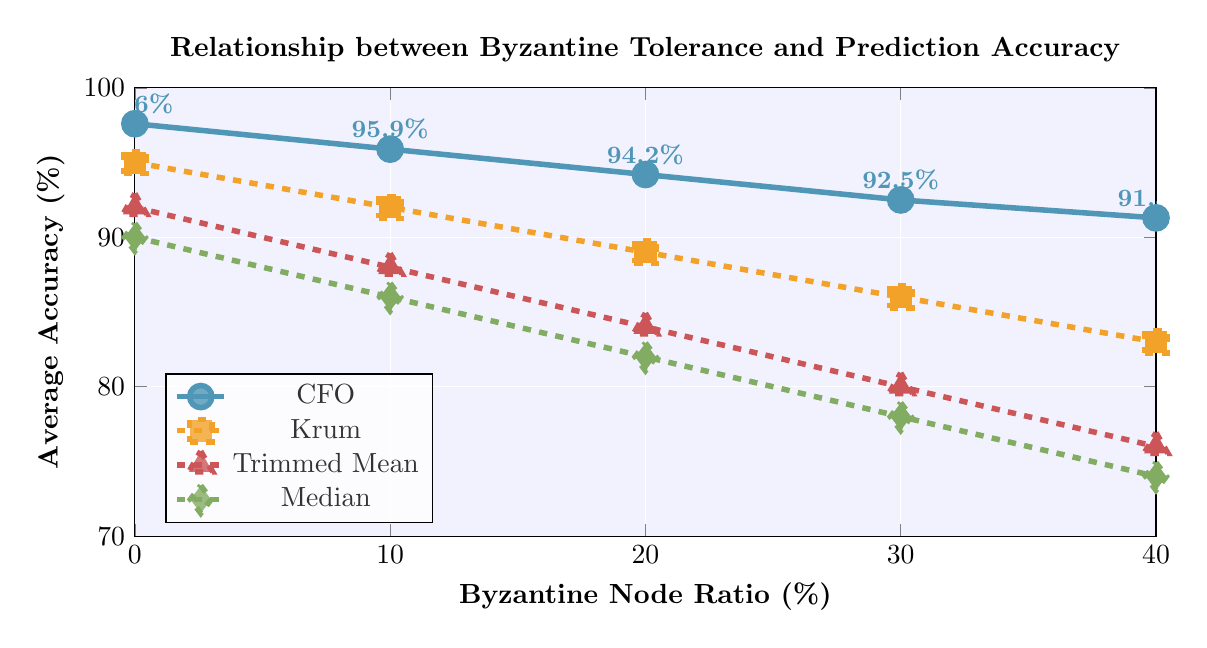
\begin{tikzpicture}
\begin{axis}[
    title={\textbf{Relationship between Byzantine Tolerance and Prediction Accuracy}},
    width=1.2\textwidth,
    height=0.6\textwidth,
    xmin=0, xmax=40,
    ymin=70, ymax=100,
    xmajorgrids=true,
    ymajorgrids=true,
    grid style={white},
    axis background/.style={fill=blue!5},
    xlabel={\textbf{Byzantine Node Ratio (\%)}},
    ylabel={\textbf{Average Accuracy (\%)}},
    legend pos=south west,
    legend style={fill=white, fill opacity=0.8},
    xtick={0,10,20,30,40},
]

% CFO - solid line with circles
\addplot[color=colorBlue, line width=2pt, mark=*, mark size=4pt, mark options={fill=colorBlue}]
    coordinates {(0,97.6) (10,95.9) (20,94.2) (30,92.5) (40,91.3)};
\addlegendentry{CFO}
\node[above, color=colorBlue, font=\bfseries\small] at (axis cs:0,97.6) {97.6\%};
\node[above, color=colorBlue, font=\bfseries\small] at (axis cs:10,95.9) {95.9\%};
\node[above, color=colorBlue, font=\bfseries\small] at (axis cs:20,94.2) {94.2\%};
\node[above, color=colorBlue, font=\bfseries\small] at (axis cs:30,92.5) {92.5\%};
\node[above, color=colorBlue, font=\bfseries\small] at (axis cs:40,91.3) {91.3\%};

% Krum - dashed line with squares
\addplot[color=colorOrange, line width=2pt, dashed, mark=square*, mark size=4pt, mark options={fill=colorOrange}]
    coordinates {(0,95.0) (10,92.0) (20,89.0) (30,86.0) (40,83.0)};
\addlegendentry{Krum}

% Trimmed Mean - dashed line with triangles
\addplot[color=colorRed, line width=2pt, dashed, mark=triangle*, mark size=5pt, mark options={fill=colorRed}]
    coordinates {(0,92.0) (10,88.0) (20,84.0) (30,80.0) (40,76.0)};
\addlegendentry{Trimmed Mean}

% Median - dashed line with diamonds
\addplot[color=colorGreen, line width=2pt, dashed, mark=diamond*, mark size=5pt, mark options={fill=colorGreen}]
    coordinates {(0,90.0) (10,86.0) (20,82.0) (30,78.0) (40,74.0)};
\addlegendentry{Median}

\end{axis}
\end{tikzpicture}

\end{document}
